\documentclass[oneside]{book}

\usepackage{amsmath, amsthm, amssymb, amsfonts}
\usepackage{thmtools}
\usepackage{graphicx}
\usepackage{setspace}
\usepackage{geometry}
\usepackage{float}
\usepackage{hyperref}
\usepackage[utf8]{inputenc}
\usepackage[english]{babel}
\usepackage{framed}
\usepackage[dvipsnames]{xcolor}
\usepackage{environ}
\usepackage{tcolorbox}
\tcbuselibrary{theorems,skins,breakable}
\usepackage[UTF8]{ctex}

\usepackage{quiver} % to draw commutative diagrams

\setstretch{1.2}
\geometry{
    textheight=9in,
    textwidth=5.5in,
    top=1in,
    headheight=12pt,
    headsep=25pt,
    footskip=30pt
}

% Variables
\def\notetitle{Combinatorial Mathematics Notes}
\def\noteauthor{
    by Flaricy\\
    Peking University}
\def\notedate{Spring Semester, 2024}

% The theorem system and user-defined commands
% Theorem System
% The following boxes are provided:
%   Definition:     \defn 
%   Theorem:        \thm 
%   Lemma:          \lem
%   Corollary:      \cor
%   Proposition:    \prop   
%   Claim:          \clm
%   Fact:           \fact
%   Proof:          \pf
%   Example:        \ex
%   Remark:         \rmk (sentence), \rmkb (block)
% Suffix
%   r:              Allow Theorem/Definition to be referenced, e.g. thmr
%   p:              Add a short proof block for Lemma, Corollary, Proposition or Claim, e.g. lemp
%                   For theorems, use \pf for proof blocks

% Definition
\newtcbtheorem[number within=section]{mydefinition}{Definition}
{
    enhanced,
    frame hidden,
    titlerule=0mm,
    toptitle=1mm,
    bottomtitle=1mm,
    fonttitle=\bfseries\large,
    coltitle=black,
    colbacktitle=green!20!white,
    colback=green!10!white,
}{defn}

\NewDocumentCommand{\defn}{m+m}{
    \begin{mydefinition}{#1}{}
        #2
    \end{mydefinition}
}

\NewDocumentCommand{\defnr}{mm+m}{
    \begin{mydefinition}{#1}{#2}
        #3
    \end{mydefinition}
}

% Theorem
\newtcbtheorem[use counter from=mydefinition]{mytheorem}{Theorem}
{
    enhanced,
    frame hidden,
    titlerule=0mm,
    toptitle=1mm,
    bottomtitle=1mm,
    fonttitle=\bfseries\large,
    coltitle=black,
    colbacktitle=cyan!20!white,
    colback=cyan!10!white,
}{thm}

\NewDocumentCommand{\thm}{m+m}{
    \begin{mytheorem}{#1}{}
        #2
    \end{mytheorem}
}

\NewDocumentCommand{\thmr}{mm+m}{
    \begin{mytheorem}{#1}{#2}
        #3
    \end{mytheorem}
}

% Lemma
\newtcbtheorem[use counter from=mydefinition]{mylemma}{Lemma}
{
    enhanced,
    frame hidden,
    titlerule=0mm,
    toptitle=1mm,
    bottomtitle=1mm,
    fonttitle=\bfseries\large,
    coltitle=black,
    colbacktitle=violet!20!white,
    colback=violet!10!white,
}{lem}

\NewDocumentCommand{\lem}{m+m}{
    \begin{mylemma}{#1}{}
        #2
    \end{mylemma}
}

\newenvironment{lempf}{
	{\noindent{\it \textbf{Proof for Lemma}}}
	\tcolorbox[blanker,breakable,left=5mm,parbox=false,
    before upper={\parindent15pt},
    after skip=10pt,
	borderline west={1mm}{0pt}{violet!20!white}]
}{
    \textcolor{violet!20!white}{\hbox{}\nobreak\hfill$\blacksquare$} 
    \endtcolorbox
}

\NewDocumentCommand{\lemp}{m+m+m}{
    \begin{mylemma}{#1}{}
        #2
    \end{mylemma}

    \begin{lempf}
        #3
    \end{lempf}
}

% Corollary
\newtcbtheorem[use counter from=mydefinition]{mycorollary}{Corollary}
{
    enhanced,
    frame hidden,
    titlerule=0mm,
    toptitle=1mm,
    bottomtitle=1mm,
    fonttitle=\bfseries\large,
    coltitle=black,
    colbacktitle=orange!20!white,
    colback=orange!10!white,
}{cor}

\NewDocumentCommand{\cor}{+m}{
    \begin{mycorollary}{}{}
        #1
    \end{mycorollary}
}

\newenvironment{corpf}{
	{\noindent{\it \textbf{Proof for Corollary.}}}
	\tcolorbox[blanker,breakable,left=5mm,parbox=false,
    before upper={\parindent15pt},
    after skip=10pt,
	borderline west={1mm}{0pt}{orange!20!white}]
}{
    \textcolor{orange!20!white}{\hbox{}\nobreak\hfill$\blacksquare$} 
    \endtcolorbox
}

\NewDocumentCommand{\corp}{m+m+m}{
    \begin{mycorollary}{}{}
        #1
    \end{mycorollary}

    \begin{corpf}
        #2
    \end{corpf}
}

% Proposition
\newtcbtheorem[use counter from=mydefinition]{myproposition}{Proposition}
{
    enhanced,
    frame hidden,
    titlerule=0mm,
    toptitle=1mm,
    bottomtitle=1mm,
    fonttitle=\bfseries\large,
    coltitle=black,
    colbacktitle=yellow!30!white,
    colback=yellow!20!white,
}{prop}

\NewDocumentCommand{\prop}{+m}{
    \begin{myproposition}{}{}
        #1
    \end{myproposition}
}

\newenvironment{proppf}{
	{\noindent{\it \textbf{Proof for Proposition.}}}
	\tcolorbox[blanker,breakable,left=5mm,parbox=false,
    before upper={\parindent15pt},
    after skip=10pt,
	borderline west={1mm}{0pt}{yellow!30!white}]
}{
    \textcolor{yellow!30!white}{\hbox{}\nobreak\hfill$\blacksquare$} 
    \endtcolorbox
}

\NewDocumentCommand{\propp}{+m+m}{
    \begin{myproposition}{}{}
        #1
    \end{myproposition}

    \begin{proppf}
        #2
    \end{proppf}
}

% Claim
\newtcbtheorem[use counter from=mydefinition]{myclaim}{Claim}
{
    enhanced,
    frame hidden,
    titlerule=0mm,
    toptitle=1mm,
    bottomtitle=1mm,
    fonttitle=\bfseries\large,
    coltitle=black,
    colbacktitle=pink!30!white,
    colback=pink!20!white,
}{clm}


\NewDocumentCommand{\clm}{m+m}{
    \begin{myclaim*}{#1}{}
        #2
    \end{myclaim*}
}

\newenvironment{clmpf}{
	{\noindent{\it \textbf{Proof for Claim.}}}
	\tcolorbox[blanker,breakable,left=5mm,parbox=false,
    before upper={\parindent15pt},
    after skip=10pt,
	borderline west={1mm}{0pt}{pink!30!white}]
}{
    \textcolor{pink!30!white}{\hbox{}\nobreak\hfill$\blacksquare$} 
    \endtcolorbox
}

\NewDocumentCommand{\clmp}{m+m+m}{
    \begin{myclaim*}{#1}{}
        #2
    \end{myclaim*}

    \begin{clmpf}
        #3
    \end{clmpf}
}

% Fact
\newtcbtheorem[use counter from=mydefinition]{myfact}{Fact}
{
    enhanced,
    frame hidden,
    titlerule=0mm,
    toptitle=1mm,
    bottomtitle=1mm,
    fonttitle=\bfseries\large,
    coltitle=black,
    colbacktitle=purple!20!white,
    colback=purple!10!white,
}{fact}

\NewDocumentCommand{\fact}{+m}{
    \begin{myfact}{}{}
        #1
    \end{myfact}
}


% Proof
\NewDocumentCommand{\pf}{+m}{
    \begin{proof}
        [\noindent\textbf{Proof.}]
        #1
    \end{proof}
}

% Example
\newenvironment{example}{%
    \par
    \vspace{5pt}
	\begin{minipage}{\textwidth}
		\noindent\textbf{Example.}
		\tcolorbox[blanker,breakable,left=5mm,parbox=false,
	    before upper={\parindent15pt},
	    after skip=10pt,
		borderline west={1mm}{0pt}{cyan!10!white}]
}{%
		\endtcolorbox
	\end{minipage}
    \vspace{5pt}
}

\NewDocumentCommand{\ex}{+m}{
    \begin{example}
        #1
    \end{example}
}


% Remark
\NewDocumentCommand{\rmk}{+m}{
    {\it \color{blue!50!white}#1}
}

\newenvironment{remark}{
    \par
    \vspace{5pt}
    \begin{minipage}{\textwidth}
        {\par\noindent{\textbf{Remark.}}}
        \tcolorbox[blanker,breakable,left=5mm,
        before skip=10pt,after skip=10pt,
        borderline west={1mm}{0pt}{cyan!10!white}]
}{
        \endtcolorbox
    \end{minipage}
    \vspace{5pt}
}

\NewDocumentCommand{\rmkb}{+m}{
    \begin{remark}
        #1
    \end{remark}
}


\newcommand{\lcm}{\operatorname{lcm}}



% ------------------------------------------------------------------------------

\begin{document}
% \begin{CJK}{GBK}{song}

\title{\textbf{
    \LARGE{\notetitle} \vspace*{10\baselineskip}}
    }
\author{\noteauthor}
\date{\notedate}

\maketitle
\newpage

\tableofcontents
\newpage

% ------------------------------------------------------------------------------

\chapter{Examples 标题}

\section{Theorem System}

\defn{Definition Name}{
    A defintion.
    中文测试
}

\thmr{Theorem Name}{mybigthm}{
    A theorem.
}

\lem{Lemma Name}{
    A lemma.
}

\fact{
    A fact.
}

\cor{
    A corollary.
}

\prop{
    A proposition.
}

\clmp{}{
    A claim.
}{
    A reference to Theorem~\ref{thm:mybigthm}
}

\pf{
    Veniam velit incididunt deserunt est proident consectetur non velit ipsum voluptate nulla quis. Ea ullamco consequat non ad amet cupidatat cupidatat aliquip tempor sint ea nisi elit dolore dolore. 

    Laboris labore magna dolore eiusmod ea ex et eiusmod laboris. Et aliquip cupidatat reprehenderit id officia pariatur. 
}

\eg{
    Nostrud esse occaecat Lorem dolore laborum exercitation adipisicing eu sint sunt et. Excepteur voluptate consectetur qui ex amet esse sunt ut nostrud qui proident non. Ipsum nostrud ut elit dolor. Incididunt voluptate esse et est labore cillum proident duis.
}

\rmk{
    Some remark.
}

\rmkb{
    Some more remark.
}

\section{Pictures}

\begin{figure}[H]
    \center
    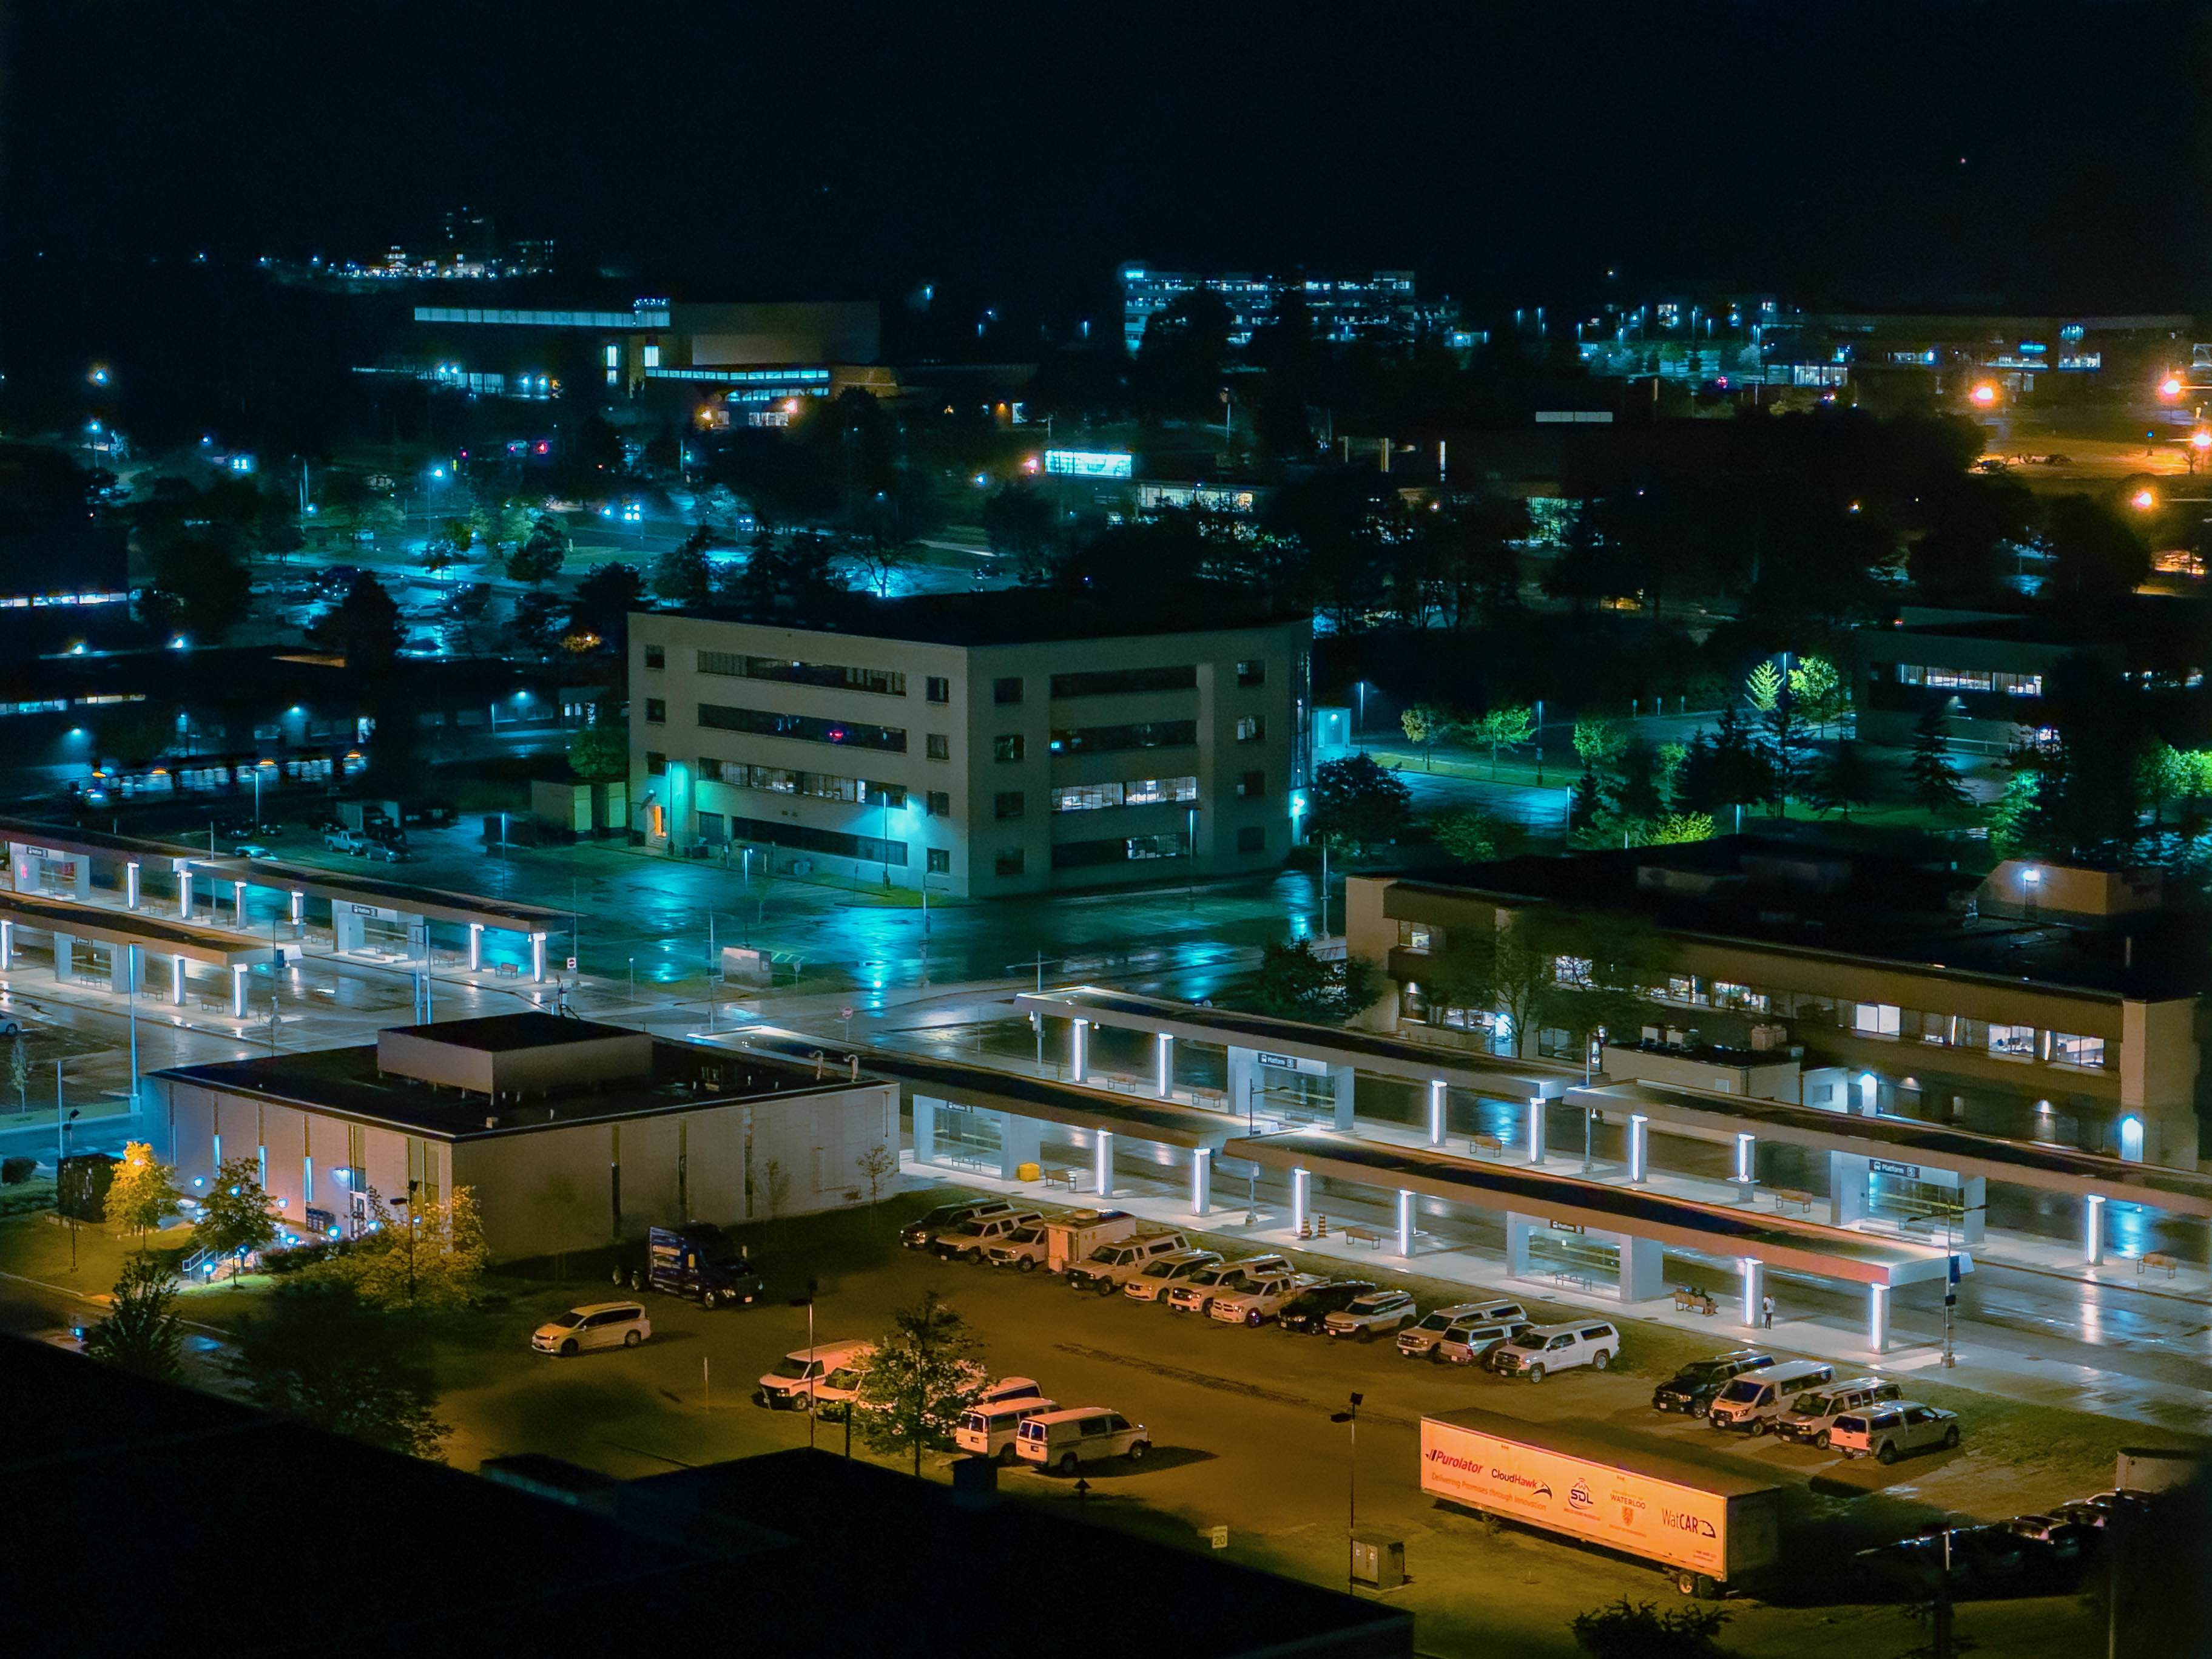
\includegraphics[scale=0.1]{img/loo.jpg}
    \caption{Waterloo, ON}
\end{figure}


\chapter{组合存在性定理}

\section{有限偏序集的分解定理(Dilworth's Theorem)}

{\it to be written}

\section{Pigeonhole Principle}
\ex{
    从1到2n的正整数中,任取n+1个数,至少有一对数,其中一个数是另一个数的倍数。
}

\pf{
    考虑将每个数分解成 $a_i = 2^{b_i}r_i, i = 1,2,...,n+1$. 由于 $1~2n$
    中仅有 $n$ 个数,所以存在 $i<j, r_i = j_j$, 则必有 $a_i | a_j$ 或者 $a_j | a_i$.
}

\ex{
    任意 m 个有序的数中存在连续若干个的和是 m 的倍数。
}
\pf{
    考虑前缀和 mod m 的余数即可。
}

\ex{
    $a_1,...,a_{n^2+1}$ 是实数序列,证明:可以选出 $n+1$ 个元素的子序列使得单调增或者单调减。
}


\pf{
    假设选不出长度为 $n+1$ 的单调序列。令 $m_i$ 表示以$a_i$ 为第一个元素的单调{\bf 增}子序列的最长的长度,则 $m_i \le n$. 
    由抽屉原理,存在 $n+1$ 个下标 $i_1,...,i_{n+1}$ 使得 $m_{i_1}=...=m_{i_{n+1}}$.
    如果存在 $1\le s<t\le n+1$, 使得 $a_{i_s} \le a_{i_t}$,则以 $a_{i_s}$ 开头的单调序列可以更长。矛盾。

    因此 $a_{i_1} > a_{i_2} > ... > a_{i_{n+1}}$, 我们得到长度为 $n+1$ 的严格递减序列。
}
\section{Ramsey's Theorem}

一种简单形式,
\prop{红蓝染色$K_9$的边,证明存在红色的$K_4$或蓝色的$K_3$。By convention, $K_n$ is the complete graph of order $n$.}
\begin{proof}
    Claim: 存在一个节点关联至少4条蓝边或者6条红边。

    若否,则图中红边数量不超过 $[\frac{5 \times 9}{2}] = 22$, 蓝边数量不超过 $[\frac{3\times 9}{2}] = 13$, 但是 $K_9$ 有 $C_9^2 = 36$ 条边。矛盾。

    如果 $v_1$ 关联了4条蓝色边,
    \[\begin{tikzcd}
        && {v_1} \\
        \bullet &&&& \bullet \\
        & \bullet && \bullet
        \arrow[color={rgb,255:red,92;green,92;blue,214}, no head, from=1-3, to=2-1]
        \arrow[color={rgb,255:red,92;green,92;blue,214}, no head, from=1-3, to=2-5]
        \arrow[color={rgb,255:red,92;green,92;blue,214}, no head, from=1-3, to=3-2]
        \arrow[color={rgb,255:red,92;green,92;blue,214}, no head, from=1-3, to=3-4]
    \end{tikzcd}\]

    如果上图中4个点之间存在蓝色边,则出现蓝色$K_3$. 若都是红色边,则出现红色$K_4$.

    如果 $v_1$ 关联了6条红色边,考虑这6个点之间的染色,
    \[\begin{tikzcd}
        \bullet && {v_1} && \bullet \\
        \bullet &&&& \bullet \\
        & \bullet && \bullet
        \arrow[color={rgb,255:red,214;green,92;blue,92}, no head, from=1-1, to=1-3]
        \arrow[color={rgb,255:red,214;green,92;blue,92}, no head, from=1-3, to=1-5]
        \arrow[color={rgb,255:red,214;green,92;blue,92}, no head, from=1-3, to=2-1]
        \arrow[color={rgb,255:red,214;green,92;blue,92}, no head, from=1-3, to=2-5]
        \arrow[color={rgb,255:red,214;green,92;blue,92}, no head, from=1-3, to=3-2]
        \arrow[color={rgb,255:red,214;green,92;blue,92}, no head, from=1-3, to=3-4]
    \end{tikzcd}\]
    
    由于2-染色$K_6$必定出现红色或蓝色$K_3$. 如果出现蓝色$K_3$,已经证毕。如果出现红色$K_3$,则和$v_1$组成红色$K_4$.
\end{proof}

\prop{$K_8$不满足上个命题的性质}
\begin{proof}
    \[\begin{tikzcd}
        & \bullet & \bullet \\
        \bullet &&& \bullet \\
        \bullet &&& \bullet \\
        & \bullet & \bullet
        \arrow[color={rgb,255:red,214;green,92;blue,92}, no head, from=1-2, to=1-3]
        \arrow[color={rgb,255:red,214;green,92;blue,92}, no head, from=1-2, to=2-1]
        \arrow[color={rgb,255:red,214;green,92;blue,92}, no head, from=1-2, to=2-4]
        \arrow[color={rgb,255:red,214;green,92;blue,92}, no head, from=1-2, to=3-1]
        \arrow[color={rgb,255:red,214;green,92;blue,92}, no head, from=1-3, to=2-4]
        \arrow[color={rgb,255:red,214;green,92;blue,92}, no head, from=1-3, to=3-4]
        \arrow[color={rgb,255:red,214;green,92;blue,92}, no head, from=2-1, to=1-3]
        \arrow[color={rgb,255:red,214;green,92;blue,92}, no head, from=2-1, to=3-1]
        \arrow[color={rgb,255:red,214;green,92;blue,92}, no head, from=2-1, to=4-2]
        \arrow[color={rgb,255:red,214;green,92;blue,92}, no head, from=2-4, to=3-4]
        \arrow[color={rgb,255:red,214;green,92;blue,92}, no head, from=2-4, to=4-3]
        \arrow[color={rgb,255:red,214;green,92;blue,92}, no head, from=3-1, to=4-2]
        \arrow[color={rgb,255:red,214;green,92;blue,92}, no head, from=3-4, to=4-2]
        \arrow[color={rgb,255:red,214;green,92;blue,92}, no head, from=4-2, to=4-3]
        \arrow[color={rgb,255:red,214;green,92;blue,92}, no head, from=4-3, to=3-1]
        \arrow[color={rgb,255:red,214;green,92;blue,92}, no head, from=4-3, to=3-4]
    \end{tikzcd}\]
    除这些红色边外,其他都连蓝色边。可以验证,图中不存在蓝色三角形$K_3$,不存在红色$K_4$.
\end{proof}

上面两个命题说明9是满足此性质的最小数,$R(3,4) = 9$.

\thmr{Ramsey}{Ramsey}{
    设 $p, q$为正整数,$p, q \ge2$,则存在最小正整数$R(p, q)$,使得当$n \ge R(p, q)$时,用红蓝两色涂色$K_n$ 的
边,则或存在一个蓝色的$K_p$,或存在一个红色的 $K_q$.

}
\begin{proof}
    归纳法。不难看出 $R(p,2) = p, R(2, q) = q$.
    假设 $R(p, q-1), R(p-1,q)$ 存在,我们证明
    \[R(p,q) \le R(p,q-1) + R(p-1, q)\]
    考虑 $n = R(p,q-1) + R(p-1, q)$ 个点的图染色。任取点$v$,则或者$v$于$R(p-1,q)$个点连蓝色边,或者和$R(p,q-1)$个点连红色边(why?)。
    
    如果$v$与$R(p-1,q)$个点连蓝色边。由归纳假设,这$R(p-1,q)$个点中必存在蓝色$K_{p-1}$或红色$K_q$.若为红色$K_q$,已经结束。若为蓝色$K_{p-1}$,则和$v$组成蓝色$K_p$.

    $v$与$R(p,q-1)$个点连红色边的情况同理。
\end{proof}


% \end{CJK}
\end{document}
